\section{Secure SLP\label{sec:Secure-SLP}}
Having identified confidentiality and authorization (see \ref{sub:Confidentiality-and-Authorization}) as essential security features in open networks \citep{Cotroneo2004, Hollick2001}, this paper will outline ways to secure SLP. These protocol extensions are to be backward compatible and secured agents are to be deployable in existing networks incrementally.

\subsection{Web of Trust or Public Key Infrastructure and reputation-based trust}
Before we can start implementing confidentiality, we need to focus on the trust relationships in SLP first. As shown in \ref{sub:Authentication-and-Integrity}, SLP only supports pre-established asymmetric keys as means to trust. While this rather simplistic approach is acceptable in centrally managed networks like enterprise LANs, it is not for open networks. An open network qualifies itself as a network of nomadic devices without prior knowledge of each other. Thus mechanisms are needed that can establish trust between strangers.\\
Since SLP already comes with support for X.509 certificates, it appears to be easiest to base trust on such keys and just eliminate the need to manually set them up and implement proper key distribution protocols instead.\\
This has been addressed by at least two well known solutions:
\begin{description}
\item [Web~of~Trust]
\end{description}
Web of Trust (WOT) is a concept to create trust between peers in a network and is an alternative to a Public Key Infrastructure model. WOT is based on a decentralized structure so there is no central authority needed and it is operating with public-key cryptography. Both are parts of an open network using service discovery with SLP. In Web of Trust a user A establishes trust to user B while sign B's public key with his private key. In that way other users can verify that A is trusting B. Trust in WOT has also a transitive relation. That means if user A trust user B then user A automatically trust everyone trusted by user B. Problem arises if a user revokes his trust. In that case other network peers don't get this information immediately like in PKI. So a potential vicious user can act at least a short time as a trustworthy person. This kind of trust would work well while SLP is in directory-less mode. 
\begin{description}
\item [Public~Key~Infrastructure]
\end{description}
Public Key Infrastructure is a concept to create trust between peers in a network. It is based on public-key cryptography and provides a centralized architecture. PKI requires at least one server which has to be reachable all the time and which has to provide several instances (registration, certificate and validation authority) so other users can request new and/or verify other certificates in real time. In some cases it is possible but quite difficult to provide a PKI in an open network so alternatives like Web of Trust are needed. To manage a PKI in an open network a best possibility is to have internet access, so the peers can use already available PKIs or to have at least one fixed and foremost trustworthy peer who could act as a server. Otherwise PKIs are nonsensically in an open network. This kind of trust requires a centralized structure, so it would just work while SLP is in directory-based mode. Both technologies solve the key distribution protocol successfully. However each has its own shortcoming in open networks.\\\\
To balance off said shortcomings a reputation-based trust model may be used on top of static key-based trust models. Reputation-based trust takes the agent behavior\footnote{E.g. amount of network messages sent} over time into account. It then uses its behavior as input parameters for a continuous function that marks trustworthiness, indifference or mistrust of the agent. The key-based model is used to bootstrap the reputation-based model by means of recommendation. A detailed definition of a reputation-based trust model can be found in Secure Pervasive Discovery Protocol (SPDP) \citep{Almenarez2003}.\\
However in cases where devices are resource constrained by battery lifetime, a reputation based trust model might not be feasible at all. In order to measure peer behavior, a device needs to constantly monitor the network or listen for reputation related trust notifications by other peers. This prevents the device from hibernating to save energy. Moving this functionality off to infrastructure services is only possible if the open network provides such services.

\subsection{Confidentiality via Security Groups\label{sub:Confidentiality-via-Security}}
Once a reliable and usable trust relationship has been established we can use it to create Security Groups (SGs) among those agents. SGs have been proposed by \citet{Hollick2001}. A SG is a group of agents which share a common secret (symmetric key). This key is used to encrypt all communication between each other. Due to the fact that the same two peers might be part of different SGs, the key association cannot be based on the sender address alone\footnote{Unless each SG uses a unique multicast group and or port}. Therefore complete encryption of the SLP message payload would not only cause severe performance penalties for non SG members, but force group members to try all associated keys in worst case scenarios. Thus \citet{Hollick2001} suggests to revert to Internet layer encryption by using Internet Protocol Security (IPSec) \citep{Kent2005} for peer communication. Group communication is left open though. This paper takes a different approach and uses application layer encryption on top of Internet layer multicast. This alleviates the network requirements and handles security within SLP entirely. Additionally this allows reusing multicast encryption for unicast channels as well\footnote{Unicast may reuse the group share secret in SLP}.\\
\citet{Huang2007} discuss various approaches to secure group communication with multicast. All of these Group Key Agreement protocols (GKA) suffer from two basic security implications that differ from point-to-point communication \citep{Prakash2008}:
\begin{description}
\item [One~affects~all] The compromise of a single group member affects the security of the whole group
\item [Re-keying~on~leave/join] No past/future data is allowed to be decrypt-able by future/past group members
\end{description}
In the scope of this paper the first problem can only be addressed by allowing a group member to request a group key renewal once a compromise has been detected. On the other hand this might open the door to availability attacks if a group member spams the SG with re-keying requests. A viable countermeasure to would be a burst rate that limits a peer's capability of request key renewal.\\
Regarding the second security implication, this paper argues that it can be relaxed in the scope of SLP to simplify the encryption protocol overhead significantly. Unless a new SA joins a SG or an existing SA incrementally updates its service description\footnote{Subsequently incremental updates will be seen as SG re-joins}, the SG's data is stale. A former group member does not learn anything new. Thus, only a change of a SA membership requires re-keying to exchange the group key. This also limits the effects of a compromise of group member (in at least very active) SGs where constant re-keying occurs regularly.\\
Open networks pose two more constraints on the group encryption protocol. The protocol must not require group members to know each other. Nor is a centralized architecture acceptable as it would introduce a single point of failure.\\
An agent has to be trusted by a member of the security group to join it. Optionally authorization can be enforced during group joining. SGs can be created by all agent types, though since advertising a SG has to be made with traditional SLP, an initiator of a SG always needs to assume the role of a SA anyway.

\subsection{Initiating a Security Group}
\begin{figure}[!h]
\centering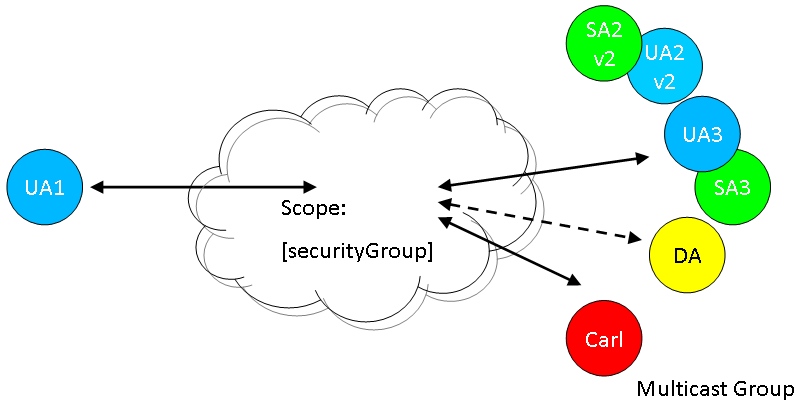
\includegraphics[width=0.5\textwidth]{Images/security-group_scope}
\caption{\label{fig:SecurityGroup-Scope}A dedicated scope denoting security groups. Since SG-advertisements are sent out using unencrypted SLPv2, attackers (Carl) are capable to discover SGs. However this does not pose a security threat.}
\end{figure}\noindent
Introducing SGs poses a chicken and egg problem on SecureSLP. How does a peer learn of the existence of a SG? Fortunately the functionality provided by traditional SLPv2 can be leveraged to advertise SGs via unencrypted service advertisements. However this allows an attacker to discover all available SGs. While the attacker will not be able to join the SG, it is essential that the advertisement does not leak confidential information as part of the service description. The only information which is essentially required is an SG identification that is best represented by public-key of the SG initiator.\\
Using a special service type that denotes a SG is one possibility how to make SGs discoverable by agents. This paper however takes a different approach and assigns a new keyword that marks a dedicated scope for SGs. This is favorable to a special service type since it practically hides SGs from legacy SLPv2 agents that would not be able to interact with a SG anyway (see \ref{sub:Protocols-basics}). Figure \ref{fig:SecurityGroup-Scope} depicts SG advertisement. The right side shows agents which are part of the same multicast group with the UA1 that queries for SGs. Agents marked with \emph{v2} ignore the query as it is not send to the default scope and are both not configured for the special scope explicitly.

\subsection{Security Groups and Directory Agents}
As stated earlier in this paper, DAs cause security implications for the security of SLP, which have to be accounted for. \citet{Hollick2001} does not address this topic and simply assumes the non-existence of DAs. This assumption is untenable in SLP as the fallback to DA mode is built into the protocol and UAs and SAs are required to use a DA if present (see \ref{sub:Protocols-basics}). Even though a forged DA would not be able to tamper with service descriptions due to integrity checks, it can prevent SGs from being established by silently discarding SG advertisements. Therefore SLP agents must revert to multicast convergence if a DA cannot be authenticated to be legit.\\
In case a DA is to be used together with SGs, it has to become a member of each and every group in the network. Otherwise it will not be able to decrypt the service description and answer queries sent by UAs.\\\\
The previous requirement and the ones listed in \ref{sub:Confidentiality-via-Security} make the Group Diffie-Hellman (GDH) outlined in \citet{Bhaskar2007} a good candidate as a GKA for SecureSLP.